% V2 manuscript insertion. The original main.tex is not modified.

\begin{figure*}[!t]
  \centering
  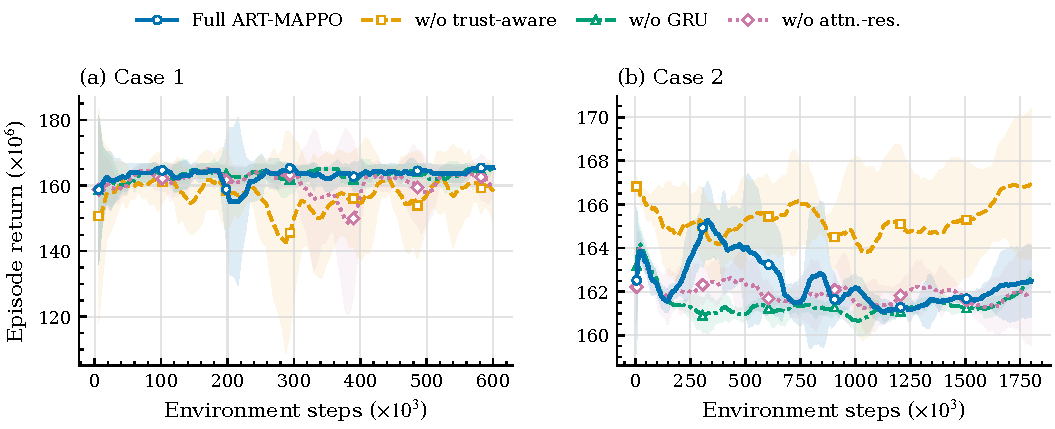
\includegraphics[width=\textwidth]{V2/figures/ablation_training_reward.pdf}
  \caption{Reward learning curves of the ART-MAPPO component ablation in
  Cases 1 and 2. Solid/dashed lines denote the five-seed mean and shaded
  regions denote 95\% Student-\(t\) confidence intervals. A common trailing
  moving average equal to 5\% of each training horizon is used for visual
  clarity.}
  \label{fig:ablation_training_reward}
\end{figure*}

\begin{figure*}[!t]
  \centering
  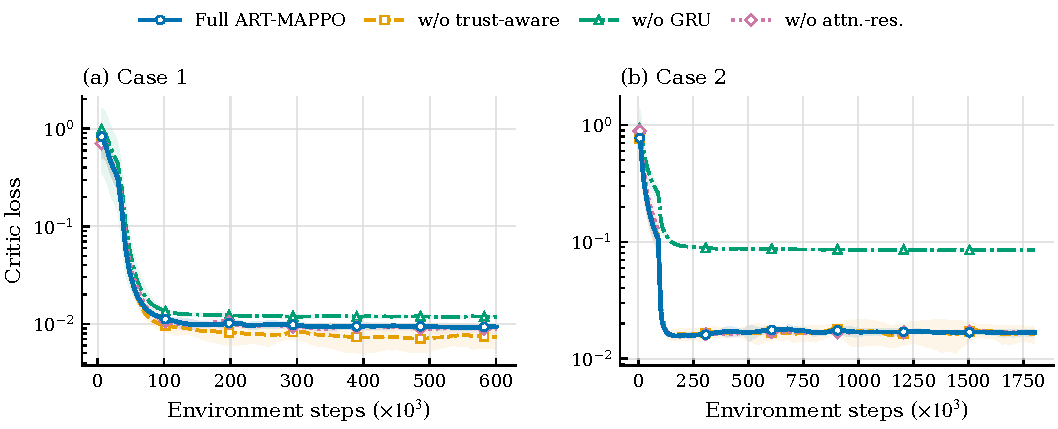
\includegraphics[width=\textwidth]{V2/figures/ablation_critic_loss.pdf}
  \caption{Critic-loss learning curves of the ART-MAPPO component ablation.
  Removing the GRU produces a persistent value-estimation error in Case 2,
  whereas the full recurrent model converges to the same low-loss region as
  the other recurrent variants.}
  \label{fig:ablation_critic_loss}
\end{figure*}

\begin{figure*}[!t]
  \centering
  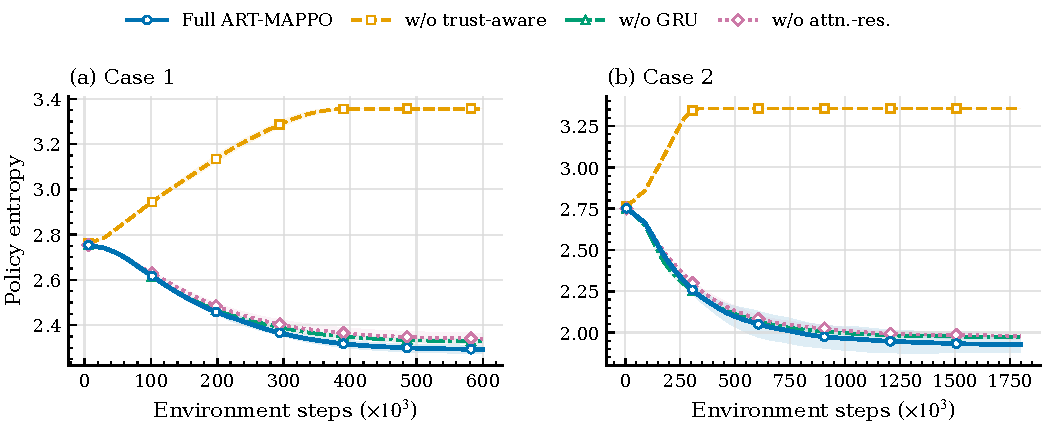
\includegraphics[width=\textwidth]{V2/figures/ablation_policy_entropy.pdf}
  \caption{Policy-entropy learning curves of the ART-MAPPO component
  ablation. Trust-aware training yields a gradual transition from exploration
  to exploitation, whereas the no-trust policy remains at high entropy.}
  \label{fig:ablation_policy_entropy}
\end{figure*}

\subsubsection{Component-ablation analysis}
We align each ablation criterion with the role of the corresponding module.
Trust-aware exploration is a training-time mechanism and is therefore
evaluated primarily through entropy evolution and cross-seed learning
stability. Full ART-MAPPO reduces policy entropy from 2.7201 to 2.2947 in
Case 1 and from 2.5615 to 1.9280 in Case 2, whereas the no-trust variant rises
to and remains at 3.3568. The pooled entropy-reduction difference is
significant after Holm correction ($d_z=22.83$,
$p_{\mathrm{Holm}}=0.00586$). In Case 1, removing trust also increases the
tail-return standard deviation from $0.396\times10^6$ to
$6.173\times10^6$, supporting the intended exploration--exploitation and
training-stability roles.

The GRU and attention--residual backbone are active during both learning and
inference, and are consequently assessed at both stages. Removing the GRU
increases tail critic loss from 0.009283 to 0.011848 in Case 1 and from
0.016745 to 0.085215 in Case 2. This lower-loss advantage is significant
across the ten matched seed--case pairs ($d_z=1.022$,
$p_{\mathrm{Holm}}=0.00586$), indicating more accurate value estimation from
temporal engagement history. Its terminal Monte Carlo contribution is mixed,
however, and the no-GRU policy remains competitive under the current
observation design.

Removing the attention--residual backbone reduces the pooled tail return by
$1.709\times10^6$ ($d_z=0.884$,
$p_{\mathrm{Holm}}=0.0469$). This training effect is directionally consistent
with the post-training evaluation: in Case 1, strict interception and
coordination decrease from 100\%/90\% to 98\%/81\%; in Case 2, per-target
interception and coordination decrease from 44.625\%/30.5\% to
38.625\%/23.625\%. The replacement MLP is parameter matched, isolating the
topological contribution of attention and residual feature processing.

Post-training results use 100 deterministic held-out Monte Carlo trials per
variant and case, comprising 20 trials for each of five independently trained
seeds. The strict all-target Case-2 metric has a floor effect for every
variant; it is retained in the reported tables, while per-target rates are
used only as secondary diagnostics.
